%%%%%%%%%%%%%%%%%%%%%%%%%%%%%%%%%%%%%%%%%%%%%%%%%%%%%%%%%%%%%%%%%%%%%%%%%%%%%%%%%%%%%%%%%%%%%%%%%%%%%%%%%%%%%%%%%%%%%%%%%%%%%%%%%%%%%%%%%%%%%%%%%%%%%%%%%%%
% This is just an example/guide for you to refer to when submitting manuscripts to Frontiers, it is not mandatory to use Frontiers .cls files nor frontiers.tex  %
% This will only generate the Manuscript, the final article will be typeset by Frontiers after acceptance.   
%                                              %
%                                                                                                                                                         %
% When submitting your files, remember to upload this *tex file, the pdf generated with it, the *bib file (if bibliography is not\daleth  within the *tex) and all the figures.
%%%%%%%%%%%%%%%%%%%%%%%%%%%%%%%%%%%%%%%%%%%%%%%%%%%%%%%%%%%%%%%%%%%%%%%%%%%%%%%%%%%%%%%%%%%%%%%%%%%%%%%%%%%%%%%%%%%%%%%%%%%%%%%%%%%%%%%%%%%%%%%%%%%%%%%%%%%

%%% Version 3.4 Generated 2022/06/14 %%%
%%% You will need to have the following packages installed: datetime, fmtcount, etoolbox, fcprefix, which are normally inlcuded in WinEdt. %%%
%%% In http://www.ctan.org/ you can find the packages and how to install them, if necessary. %%%
%%%  NB logo1.jpg is required in the path in order to correctly compile front page header %%%

\documentclass[utf8]{FrontiersinVancouver} 
\usepackage{url,hyperref,lineno,microtype,subcaption,framed, float, dirtytalk, amsmath, tikz, svg, svg-extract}
\usepackage[onehalfspacing]{setspace}
\newcommand\tab[1][1cm]{\hspace*{#1}}

\linenumbers
% Leave a blank line between paragraphs instead of using \\ 


\def\keyFont{\fontsize{8}{11}\helveticabold}
\def\firstAuthorLast{van Steenbergen} %use et al only if is more than 1 author
\def\Authors{Maas van Steenbergen\,$^{1,*}$}
% Affiliations should be keyed to the author's name with superscript numbers and be listed as follows: Laboratory, Institute, Department, Organization, City, State abbreviation (USA, Canada, Australia), and Country (without detailed address information such as city zip codes or street names).
% If one of the authors has a change of address, list the new address below the correspondence details using a superscript symbol and use the same symbol to indicate the author in the author list.
\def\Address{$^{1}$ Faculty of Behavioural and Social Sciences,  Methodology \& Statistics, Utrecht University, the Netherlands  }
% The Corresponding Author should be marked with an asterisk
% Provide the exact contact address (this time including street name and city zip code) and email of the corresponding author
\def\corrAuthor{Corresponding Author}

\def\corrEmail{m.vansteenbergen@uu.nl}


\begin{document}
\onecolumn
\firstpage{1}

\title[]{Aggregated Rating Scale Scores Are Not Ordinal} 

\author[\firstAuthorLast]{\Authors} %This field will be automatically populated
\address{} %This field will be automatically populated
\correspondance{} %This field will be automatically populated

\extraAuth{}% If there are more than 1 corresponding author, comment this line and uncomment the next one.
%\extraAuth{corresponding Author2 \\ Laboratory X2, Institute X2, Department X2, Organization X2, Street X2, City X2 , State XX2 (only USA, Canada and Australia), Zip Code2, X2 Country X2, email2@uni2.edu}

\maketitle

%%% Leave the Abstract empty if your article does not require one, please see the Summary Table for full details.

\begin{quote}
    ``\textit{Eh bien!}''--exclaimed Walras characteristically--``this difficulty is not insurmountable. Let us suppose that this measure exists, and we shall be able to give an exact and mathematical account of it''.\ 
    [\dots]\ In view of the fact that theoretical science is a living organism, it would not be exaggerating to say that this attitude is tantamount to planning a fish hatchery in a moist flower bed''.\\
    \textit{-- Nicholas Georgescu-Roegen}

\end{quote}
\begin{quote}
    ``I think the foundations of measurements [\ldots] have a lot of implications about the way you do and actually think about measurement. There is a great deal of feedback from work on foundations on the actual practice, unlike a lot of other fields of mathematics, where work on foundations is divorced from the practice of other disciplines''.\\
    \textit{-- Amon Tversky}
\end{quote}

\section{Introduction}
Variables in psychology often aim to quantify strength of sensation, personality traits, or attitudes. Because such variables are based on subjective feelings and opinion, they cannot be measured directly. We cannot look in the heads and experience what they experience. This means that research participants need to communicate their `state' of a variable of interest in ways that allow for statistical analysis. Many tools are invented that entice research participants to produce numerical estimates of sensations, personality trains, and attitudes in a systematic manner. The rating scale is the most popular family of instruments by far. This family of instruments always involves a series of ordered options that represent an increasing magnitude on a variable of interest. Its strengths include its low price of administration, the easy reproducability, and its similar appearence in different modalities. 

Yet, estimates that are gained through these methods are different from what is commonly understood by measurement. Scoring `extremely likely', `4' or `very often' on a rating instrument does not have the same unambiguous meaning as a read-out of 5.2 cm on a piece of measuring tape. There is a clear contrast between estimates of psychological variables with the measures of length, of temperature, or of weight. When we measure with a measuring tape the value of the measure is uniquely determined in every regard, aside from its scale, which is chosen by convention. A rating scale response is less constrained than that: we know that `very often' is more than `often', but not how much more often `very often' is as compared to `often'.

This difference has traditionally been understood within psychology as the difference between ordinal scales on the one hand, and interval- or ratio-level scales on the other hand. This distinction was introduced by the psychologist Stevens. When an attribute is ordinal, we know that the scores can only say something about relative ordering: we know that `very likely' is higher than `likely'. With interval- and ratio-level scales, the empirical relationships are expressed in terms of the ratio of the attribute of one object to a standard score of an attribute: the unit. Stevens saw the measurement as the `assignment of numerals to objects according to rule'. There were different levels of stringentness for these rules that could be applied in different situations, and these levels of stringentness has consequences for which hypothesis testing apparatus could be applied. His theory of levels of measurement was created in response to criticism by physicists that measurement in psychology did not actually concern measurement at all. In the classical conception that predates modern psychological science, only quantitative measurement in correspondence with Hölder's axioms was considered meaningful.

Still, Stevens' solution was not very well formalized, and contained logical errors. Psychologists and philosophers of science Krantz, Luce, Suppes, and Tversky rectified many defects in the work of Stevens. Their approach was called the Representational Theory of Measurement. While they avoid giving a single definition of measurement, they explain the intention of their approach in broad strokes. They see the measurability of an object from the perspective of a representation and a uniqueness theorem. The representation theorem asserts that a set, together with one or more relations on that set, follows certain axioms so that it can truthfully preserves the structure of a qualitative attribute of an object to a numerical representation of that quality. In other words, a \textit{homomorphic} mapping of the qualitative relational structure into a quantitative representation can be constructed. A uniqueness theorem specifies the set of allowable transformations which maintain this qualitative relation strcture. E.g., both Fahrenheit or Celsius measurements are legitimate homomorphic mappings that maintain the qualitative structure of temperature, differing in zero-point and scale. More formally, suppose that the transformation function $\phi(a)$ is a homomorphism and the representation theorem holds for the mapping of qualitative ordering $\succ$ to quantitative ordering $>$. If $\phi(a)$ then maps a qualitative attribute of set A into $\mathbb{R}$, it should maintain the structure of the qualitative attribute in its numerical representation: if and only if $A$ is qualitatively greater than $B$, $a$ is numerically greater than $b$. Axiomatically, ratio-scale measurement is alligned with Hölder's axioms. It only recently started getting full attention by psychometricians as a consequence of the tireless effort of theoretical psychologists, as its difficult formalism and apparent incompatibility with psychometric methods was not initially inviting. Regardless, it is the most widely respected, formally developed, and most discussed approach to measurement in psychology. Yet, it should be known that the philosophical implications of the theory and its relevance for psychological science are under active discussion. We are adherents of `representation minimalism', where we are neutral about what empirical relations in this theory mean, but keep the formalist framework. This means that our approach is still incompatible with those commentaries that set into doubt the quantitative status of psychological variables. 

Rating scale responses are often seen as the quintessential example of ordinal measurement. Even though psychologists generally agree that ordinal rating scale responses are different from ratio-level measures, there is an ongoing discussion whether rating scales should be treated as relative-zero quantitative (interval) measures in the context of statistical testing. We argue that the picture is more complex than the choice between ratio scores and ordinal scores implied here, given that aggregations of rating scale responses are not necessarily ordinal. We also demonstrate that this can have consequences for statistical testing. To do so, we make three assumptions. The first assumption is that the rating scale score is a weakly ordered indicator of an actually existing magnitude. We also assume that the structure of the empirical relationships in nature are in correspondence with Hölder's axioms, and thus principially allows for quantitative measure. Finally, we simulate a third measure that truthfully preserves the structure of those empirical relationships. By only assuming these three characteristics, we can show that the non-ordinality of aggregates of ordinal responses can cause defects in statistical testing. By postulating that we know the magnitude of a quantity that the rating scale indicate, we can map these quantities to rating scale levels which are ordinal in nature. In the appendix, axioms for ordinality and ratio-level measurement are presented. 

For the current project, we focus our attention on cases where an attribute of interest is pricipially continuously measurable. Therefore, a \textit{homomorphic} mapping of the qualitative structure can be constructed. This mapping is a quantity: a ratio-level measurement with an absolute zero-point. We posit to know the `true value' of this attribute. We assume that the quantity of the attribute maps to the rating scale item in question. We map this quantitative representation again for each individual rating scale representation, adding different amounts of random and group-based noise to each rating scale response. Then, we apply a t-test and a Mann Whitney U-Test to all of these different mappings. We call the differences in mapping between indicators \textit{measurement instability} and make a distinction between four kinds: zero-point instability, scaling instability, and systematic and random threshold instability.\ \textit{Zero point instability} means that the relative zero-point changes between participants.\ \textit{Scaling instability} means that the distance between the zero-point and the maximum changes.\ \textit{Systematic threshold instability} means that there is a relationship between consecutive distances of pairs of thresholds. We test the robustness of these measures to measurement instability. We also present a simulation framework that can be used to study the consequences of measurement instability.

\subsubsection{Rating scales and Ordinality}
While aggregations of rating scale responses are normally understood to be ordinal, we argue that this is not true if there is between-person or within-person scaling instability. If the ordering of attributes or their relationship to the hypothetical perfect measure is not invariant to time and is not invariant between people, then the relationship of the attribute to the rating-scale representation of that attribute is not consistently weakly ordered. First, we need to explore the connection between the hypothetical perfect measure and a measure that is ordinal for one specific person at one specific time.

Assume that the empirical structure of an attribute is in correspondence with the axioms for ratio-level measurement scaling. This means, by extension, that all axioms for ordinal measurement are in correspondence with the empirical structure of that attribute. Let us assume we have a hypothetical homomorphic mapping of the empirical structure of this attribute expressed quantitatively (with ratio-scaling). Then, each possible weakly\footnote{Meaning elements can be tied, see above.} ordinal representation of quantitative values of this perfect measurement measure can result in an unambiguous weakly ordered classification of scores in $Q$ to scores in terms of $P$\footnote{This lack of ambiguity is only a result of this formalization. We may find that the relationship of the `real' variable to its ordinal estimate is not quite so straightforward. We will discuss this later on.} Assume that instrument $P$ has $n$ elements. Then we can define a series of $n - 1$ `thresholds' T as $\{ a, b, c \ldots z \}$. These thresholds are the point of $q$ where a score $p_1$ in $P$ jumps to another classification $p_2$ in $P$ on the basis of a score $q$ in $Q$. We then define a score $p$ in $P$ for each $q$ in $Q$ as follows, assuming we have an $n$-level measurement scale for $P$:

\[
\begin{cases} 
    1 & q \leq a\\
    2 & a \leq q < b\\
    3 & b \leq q < c\\
    \ldots & \ldots\\    
    n & z < q\\
\end{cases}.
\]

Note that if the mapping is inconsistent with this formalism, then the axiom of transitivity is broken: an item that is higher on a particular attribute can score lower on the scale. Thus, the form of this step function is a logical consequence of the empirical structure of the variable. It needs to be met. Otherwise, the two representations of the attribute are mutually inconsistent. Hence, the mapping function follows from the assumed structure of our hypothetical perfect representation of the variable and the assumed structure of an ordinal rating scale response. 

An ordinal representation of a continuous that groups values into a certain number of equal segments can be inconsistent with another representation of that variable that splits the range of the original variable into an identical number of equivalence sets. In fact, many different constructions can be made that are not compatible with each other. Say we want to map a continuous variable into five categories. The values of our continuous variable fall in range [0, 100] and we would like to map this range to five equivalence sets.

If so, then both

\[
p_{1} = 
\begin{cases} 
    1 & q \leq 22.4\\
    2 & 22.4 \leq q < 48.9\\
    3 & 48.9 \leq q < 59.4\\
    4 & 59.4 \leq q < 82.2\\    
    5 & 82.2 < q\\
\end{cases}
\ \ \ \text{and}\ \ \ 
p_{2} =
\begin{cases} 
    1 & q \leq 20.0\\
    2 & 20.0 \leq q < 40.0\\
    3 & 40.0 \leq q < 60.0\\
    4 & 60.0 \leq q < 80.0\\    
    5 & 80.0 < q\\
\end{cases}.
\]

are valid representations for individual rating scale scores of the variable with 5 equivalence sets. Yet, they are inconsistent, because a quantity can be sent by the mapping to one category that would be sent to another category in another mapping. E.g., the value 21.1 is seen as a 1 in the first representation while a value of 21 is seen as a 2 in the second representation. This breaks the axiom of transitivity. If we were to sum scores gained through multiple ordinal representations of the same score, the mapping becomes inconsistent between these representations. Note also that this is not equivalent to measurement error per sé, but relates to \textit{measurement instability}. The issues come to be through the incompatibility of two representations of empirical relations.

\subsection{Between-person mapping instability}
With between-person mapping instability, we refer to different incompatible representations of a continuous variable between people in a sample. 

\subsection{Time-dependent mapping instability}
People can also change in their mapping over tim. When studying within-person mappings, we can assume that those psychological processes part of Q are time-dependent. These measures are shaped by different forces and the previous states of the construct \citep{olthofComplexityPsychologicalSelfratings2020b}. Their values are continuous and are related to each other in a structured manner \citep{bokerConsequencesContinuityHunt2002}. We also assume that their values are differentiable over time, changing smoothly. Their values can increase or increase very quickly, but not instantaneously. This, they are modeled best using the rate of change of the variable, through differential equations \citep{molenaarNewPersonSpecificParadigm2009}. We assume that the mapping function of a variable develops in the same way: continuously, changing smoothly, and differentiable over time.

Making a, b, c, and d functions of time, step function F(x, t) becomes: 
\[
\begin{cases} 
    1 & q \leq a(t)\\
    2 & a(t) \leq q \leq b(t)\\
    3 & b(t) \leq q \leq c(t)\\
    \ldots & \ldots\\    
    n & z(t) \leq q\\
\end{cases}.
\]

This means that each threshold becomes a function, with time as input. 

\subsection{Measurement instability}
We introduce the \textit{measurement instability framework} to study the consequences of measuring procedures .\textit{Measurement instability} can be used to make a distinction between the influence of different parameters that affect the scaling of the mapping function. When we introduce these topics, we assume that the other measurement instability parameters are stable. We also assume equal intervals, unless otherwise specified. Note that none of the measurement instability parameters influence the quantity of the underlying variable, it only has repercussions on the mapping of the quantity to its .

\subsubsection{Zero-point instability}
\textit{Zero-point instability} means that the zero-point of the mapping is unstable. Because the absolute zero-point of the real quantity is stable, the thresholds move away or towards the absolute zero point of the real quantity by a constant amount in the same direction. The range of the thresholds will stay identical. Every threshold shifts by a constant amount. Therefore, assuming we have an $n$-level rating scale measurement scale $P$, measure $p$ is equal to:

\[
\begin{cases} 
    1 & q  \leq (a + C_{p})\\
    2 & (a + C_{p}) \leq q < (b + C_{p})\\
    3 & (b + C_{p})  \leq q < (c + C_{p})\\
    \ldots & \ldots\\    
    n & (z + C_{p})  < q\\
\end{cases}.
\]

where set of thresholds $T = \{a, b, c, \ldots, z\}$, $C_{i}$ is the constant for person or moment $p$, $a < b < c < \cdots < n$, and $q$ is a continuous measure of $Q$. 

\subsubsection{Scaling instability}
\textit{Scaling instability} is instability that comes from a changing distance between the highest threshold and the lowest threshold (the zero-point). The range of the measurement instrument is unstable. In other words, the segment of the real quantity that is mapped to the representation can be wider or more narrow in the real quantity depending on the person or the timepoint on which a person is measured. Scaling instability is independent of zero-point instability. The difference of each threshold to the lower range bound is scaled up by a common factor. Therefore, assuming we have an $n$-level rating scale measurement scale $P$, measure $p$ is equal to:

\[
\begin{cases} 
    1 & q \leq a\\
    2 & a \leq q < a + x_{p}(b - a)\\
    3 & a + x_{p}(b - a) \leq q < a + x_{p}(c - a)\\
    \cdots & \cdots\\    
    n & a + x_{p}(z - a) < q\\
\end{cases}.
\]

where where set of thresholds $T = \{a, b, c, \cdots, z\}$, $x_{i}$ is the scaling factor $x$ for person or moment $p$, $a < b < c < \cdots < n$,  and $q$ is a continuous measure of $Q$.

\subsubsection{Interval instability}
\textit{Interval instability} means that the distance between consecutive pairs of thresholds is not identical. Interval instability can have a structural or a random appearence. An example of structural interval instability would be a growing distance between each subsequent neighbouring pair of thresholds. In random interval instability, there is no relationship between the order of the pairs and the distance of neighbouring pairs of thresholds. The instability is the result of random fluctuations. Interval instability can simultaneously have a structural and a random component. Assuming we have an $n$-level rating scale measurement $P$, measure $p$ is equal to:

\[
\begin{cases} 
    1 & q  \leq (a + K_{pa})\\
    2 & (a + K_{pa}) \leq q < (b + K_{pb})\\
    3 & (b + K_{pb})  \leq q < (c + K_{pc})\\
    \cdots & \cdots \leq \cdots\\    
    n & (z + K_{pz}) < q\\
\end{cases}.
\]

where the set of thresholds $T = \{a, b, c, \ldots, z\}$, $K_{pt}$ is the constant for person or moment $p$ at threshold $t$, $a + K_{ia} < b + K_{ia} < \cdots < z + K_{iz}$, and $q$ is a continuous measure of $Q$.

\subsubsection{Combinations}
These three instabilities operate mostly independently but a few things should be noted. One is that real scores can fall outside of the range of the thresholds. These scores will naturally be mapped to the lowest or highest option. Second, if the zero-point of the mapping is stable then scaling instability can only affect the right bound of the range. Further, thresholds cannot be outside of the range of the measuring device by definition. Therefore, interval instability is limited by scaling and zero-point instability. We also reiterate once more that the values of the actually existing quantity are not affected by the mapping. We consider these absolute up to the point of the uniqueness theorem. Moreover, the chosen scaling of the real quantity is of no practical concern. If the original attribute would be scaled differently, it would affect the thresholds proportionately. Statistical conclusions would be identical after these scaling differences are propagated. Lastly, all forms of instability can be either systematic or unsystematic. If the instability is systematic, then the mapping of the variable from an existing quantity to the rating score is impacted by other variables of relevance to the test. If the instability is unsystematic, there is no relationship between other relevant variables and the mapping. Systematism can be consequential in the context of applying a statistical test, because if the mapping is inconsistent between test conditions it might lead to biased results. 

\section{Method}


\subsection{Aims}
The aim of this simulation is twofold. The first aim is to illustrate and clarify the potential consequences of measurement instability. The second aim is to  Given these aims, we decided to use the simplest test and data-generating mechanisms we could think of. 

\subsection{Data-generating mechanism}
Our data-generation pipeline consists of multiple stages. First, we generate the data on the data itself. 

We generate data for a simple independent-sample t-test with the aim that this test performed on the unprocessed data has a statistical power of 0.80 for a one standard deviation difference based on an $\alpha$ of 0.05. Our sample size was chosen to ensure an empirical power of 0.807: 18 participants per group.  

In the first test, the two distributions should be equivalent. Two samples are drawn from the same distribution. Therefore, our test will be rejected in 0.05 percent of cases, as should be expected. We draw both samples from a standardized normal distribution:

    \centerline{Normal ($\mu$ = 0; $\sigma$ = 1)}

In the second test, there is a one standard deviation difference between the null distribution and the alternative distribution. The parameters are as follows:


    \centerline{0:\@ Normal ($\mu = 0; \sigma = 1$)}
    \centerline{A:\@ Normal ($\mu = 1; \sigma = 1$)}

Random numbers are generated using the Xoshiro256++ algorithm. The seed is 8508845.

\subsection{Threshold transformation pipeline}
We have implemented a transformation pipeline design for which we have specified a range of parameters for each sub-type of measurement instability. These factors include the distribution of the zero-point, the number of bins the data should be divided into, the distribution of the scaling, and the distribution of the threshold distance. We emulate differences in the degree of measurement stability by running the thresholds through a transformation pipeline. Each stage of the pipeline draws on the results of the last, until one set of thresholds is left. Thresholds are generated for each iteration of the simulation, right before we perform the analysis.  

\subsubsection{Generating the zero point}
First we set a zero-point. This is based on a three standard deviation difference from the mean. If it is stable, the left bound is constant. If it is unstable, we use a normal distribution to generate a zero-point with $\mu$ is three standard deviations lower than $\mu$ is variable. In the last stage, this actual bound is cut off because the left-most category extends theoretically to lower values up to the absolute zero-point. Numbers are either a constant or drawn from a distribution. The constant is always -3. If drawn from a distribution, $\mu$ is always -3. $\sigma$ is set at each interval when incrementing by 0.1 from 0.1 to 1.0.

\subsubsection{Generating the scaling}
We placed the maximum at the right bound 3 standard deviations to the right of the mean of the null-data so that the mapping is equivalent for the two groups. The generation mechanism is similar to that of the zero-point: it is either a constant, or we use a normal distribution to generate a max-point where $\mu$ is equal to three standard deviations to the right of $\mu$. The constant is thus always 6. If drawn from a distribution, $\mu$ is always 6. $\sigma$ is set at each interval when incrementing by 0.1 from 0.1 to 1.0.

\subsubsection{Setting the number of response categories}
We set the number of response categories as one of the parameters for the simulation. This is fed into the function that generates the thresholds. The set of values includes each integer from four to fifteen, 20, 50, 80, and 100.

\subsubsection{Generating the thresholds}
We generated the intervals (all values of the thresholds aside from the outer bounds) by dividing the distance of the left bound of the range to the right bound of the range by the number of thresholds. Initially, this is always done 

Unequal thresholds were generated using the cumulative distribution function of the beta-distribution. We chose this set-up because it results in either increasing or decreasing distance between, controllable by the $\beta$-parameter. If it is stable, the same parameters are chosen for each . If it is unstable, $\alpha$ and $\beta$ were 

\subsection{Mapping the real scores to the bins}
Afterwards, we map the using the thresholds that were generated using this pipeline. 

\subsection{Analysis}
We ran two independent two-sample t-tests and two Mann-Whitney U-Tests to perform the analysis. We save the number 

\subsection{Software}
We used the Julia language, and in particular the `Statistics.jl' and `HypothesisTests.jl' packages, to set up the simulation and to run the statistical analysis \citep{bezanson2017julia}. Analyses were run on a personal computer. Full information about dependencies and version numbers can be found in a machine-readable format in the Manifest.toml file in the Github-repository. Instructions for running the analysis through a sandboxed project environment identical to our system can be found on the main page of this repository. Both the distributions and the test were chosen to use simple, commonly known statistics with the aim to show the potential consequences of zero-point, scaling, and interval instability. The experiment can be repeated using any possible test: the values are mapped \textit{before} the analysis is run, so the full study is independent of the implementation of the test.


% For Original Research articles, please note that the Material and Methods section can be placed in any of the following ways: before Results, before Discussion or after Discussion.

\section{Discussion}
The 

Another reason for the current treatment is the frustration about the limitations of modern treatments of this topic. Many modern simulation studies implicitly assume the thing that ought to be proven: that the mapping of the continuous variable to the measurement scales results in equal intervals. We believe that part of the reason for this confusion is that psychologists are allergic to making claims about the quantitativity of variables. Yet, most of the statistical tests we commonly use to test data rely on that claim. It can be difficult to understand why we rely on those assumptions for testing, but are reluctant when it comes to justification. This is an attempt to show that it can bring a great deal of clarity if we extend our lenience to allow for these assumptions when justifying them. If it turns out that this leads to silly

Our choice to give the hypothetized perfect measurement an absolute zero is based on both a defence and a justification. The justification for using the absolute zero-point (or the absence of the posited attribute) is the theoretical simplicity that is brought by an unambiguous relationship of the perfect quantity measurement and its relationship to a rating scale score.  to the common claim that one never can never really observe the absence of a value of a trait. Each quantity has to have a theoretical zero-point, because otherwise the whole idea of quantity is meaningless. Temperature, for example, does have an absolute zero-point, at 0$^\circ$ K, yet it cannot ever be reached. Nobody would argue that because temperature is  it cannot ever be reached that we should stop attempting to measure temperature in Kelvin. 

\subsection{}
The better anchored a psychological variable is to known 

\subsection{Differently Anchored Ordinal Measures}
We postulate that differences . For example, questions that directly refer to a quantity with a known scaling have negligable measurement instability. This is because there is a clear reference to the quantity and that anchors the ordinal representation to the underlying quantity. For example:

How tall are you with your shoes off?
a. 0 m --- 1.50 m
b. 1.50 m --- 1.70 m
c. 1.70 m --- 1.90 m
b. 1.90 m or taller

might not be very informative, but it has an obvious connection to the measure and is equally spaced. If an error is made, it is measurement error.

An ill-defined question can also cause issues. For example, the question

How much money do you make a month?
a. €2000 or less
a. €2000 --- €2500
b. €2500 --- €3000
c. €3000 --- €3500
c. €3500 or more,

where monthly income is defined as the net income after taxes are deducted has a larger degree of measurement instability

In another case, it is easy to imagine how to measure something, but 

\subsection{Operational ideal}

\subsection{Relationship of this framework to other theories}
We would like to 

\subsection{Relationship to Classical Test Theory}
In classical test theory, 

\subsection{Relationship to Latent Variable Theory and Measurement Invariance}
The difference between and latent variable models also deserves some attention. Both ideas relate a directly observable variable to a latent variable that cannot be directly observed. The difference is in both the intent and the underlying reasoning. Usually, latent variable models are used to relate several manifest variables to one latent construct. If I were to ask you how good you felt, there might be several  

In our simulation, we are assuming direct measures of the variables we postulate here. So:

`How satisfied are you with life on a 1 --- 10 scale?'

1 --- 2 --- 3 --- 4 --- 5 --- 6 --- 7 --- 8 --- 9 --- 10

is a measure of life satisfaction, and not an indicator of dispositional happiness. The scaling or the anchoring that people use still changes 

\subsection{Relationship to the Rasch Model}

\subsection{Validity}
We subscribe to the point of . However, we do not agree that it should be so casually treated as a question that can be answered with a simple yes or no. Not only the entity 

\subsection{Measurability}
The experiment above aims to show that the factors that go into scale instability, discretization, can influence. 

Some concepts are easier to measure than others. 

In the social sciences, there is often something left when you try to quantify kitchen-and-sink concepts that is not captured in the measurement. The economist Georgescu-Roegen has called this the qualitative residual \citep{georgescu-roegenMeasureQualityOptimum1965}. It is not far-fetched to assume that this qualitative residual plays a role in the difficulty of achieving scale stabiblity or defining the relative zero-point. Georgescu-Roegen asserts the importance of quantifying that residual regardless of the challenges: `We buy and sell land by acres, because land is often homogeneous over large areas; and because this homogeneity is not general, we have differential rent. How unimaginably complicated economic life would be if we adopted an ordinal measure of land chosen so as to eliminate differential rent, let alone applying the same idea to all economic variables involving qualitative variations' \citep{georgescu-roegenMeasureQualityOptimum1965}!


What is problematic, however, is that we do not know how our variables relate to 


If there is no one-to-one relationship from the measurement device to the measure, it is wise not to mistake the measurement scores for the empirical relationships that are described. This problem is called the `map-territory' problem in the philosophy of science. Rating scales were invented to make an estimate of the level of psychological variables in certain contexts, but they make a whole lot of assumptions about the nature of what those variables are. Mistaking the scores on that rating scale for the quantity of . 

Going o

It must also be said that we do feel some sympathy towards the viewpoint by Sijtsma\citep{sijtsmaPsychologicalMeasurementPhysics2012}. 

We agree with Borsboom, Mellenbergh and van Heerden that what validity should be defined as a scale measuring what it purports to measure. However, their conception is probabl. A scale might very well be able to measure what it purports to measure, but if this is only an attempt 

We align ourselves with ``representational minimalism'' that rids it of most of its epistemological basis so that it can serve as a common ground for discussion about measurement, recognizing that most of the critical literature about measurement takes place either within or in discussion of this framework \citep{vessonenRepresentationMeasurement2021}. The acceptance of RTM is not universal. We do not make firm claims whether a realist, an operationalist, or a representationalist epistemology should be matched to the formal aspects of the framework. We do, however, choose to use representationalist language, as this is the most well-known and fully realized. It should be noted that choosing a different framework means that the formalism might either change slightly or majorly. If this change is subtle, then the current study might still be interpretable. In some frameworks, however, especially those that doubt the hypothetical quantifiability of psychological constructs, the current discussion might be uninterpretable.

\subsection{Utility Measures}
An hereto unnoticed (as far as I know) strong resemblance to the discussion from economists about the status of utility measures. This problem is in many ways  identical to the problems that we see in psychology. What are the limits of 

There is a distinction between unobservable and observable properties made in psychology that pops up often, such as in the discussion of latent variables. This distinction is not without criticism. As Burgos notes, the distinction is a \citep{burgosRealProblemHypothetical2021}

\subsection{Takeaway points}
\begin{enumerate}
    \item{When thinking about measurement, it can be useful to separate \textit{measurement error} from \textit{measurement instability}. The former is an error or deviation from a measure after already assuming its scaling. The latter is caused by inconsistencies in the mapping process from the real value to its rating scale equivalents.}
    \item{The \textit{operational ideal} of the measurement instability framework is to minimize the issues that inconsistent mapping between participants or timepoints can cause. This, for example, can be through rescaling or the development of statistical measures. Moreover, uncertainty calculations can be made on the basis of estimated measurement instability.}
    \item{If it were easy to measure the relationship of the scaling of a rating scale and a `real' magnitude of a quantity, it would have been as common as }
\end{enumerate}

%%Figures, tables, and images will be published under a Creative Commons CC-BY licence and permission must be obtained for use of copyrighted material from other sources (including re-published/adapted/modified/partial figures and images from the internet). It is the responsibility of the authors to acquire the licenses, to follow any citation instructions requested by third-party rights holders, and cover any supplementary charges.

\section*{Notation}

\section*{Conflict of Interest Statement}
The authors declare that the research was conducted in the absence of any commercial or financial relationships that could be construed as a potential conflict of interest.

\section*{Funding}
No external funding was used for this project.

\section*{Acknowledgments}
I acknowledge the work of my thesis supervisors, who introduced me to the method and left me free to pursue the project as I imagined it in all its weird and shifting shapes.  The great help of the Julia community was also appreciated, as they have been pushing me forward where I got stuck and took the time to respond to my stupid questions. Finally, I would like to acknowledge the feedback and conversations between me and my thesis group, who have been working through my text and made sure that it is easy to follow and well-written. Special thanks to Giuliana Orizzonte, Daniel Anadria, dr. Hessen, dr. Derksen, dr. Grelli and dr. Bringmann for fruitful discussions and feedback about my topic. Lastly, I would like to thank my girlfriend, family, and friends for the mental support throughout.

\section*{Appendix}

\subsection{Representational Theory of Measurement}
The representational theory of measurement (RTM) is an important . While first formalized by Stevens, the most succesful 

\subsubsection{Ordinal measurement}
In this study, we assume that a single instance of a rating scale instrument results in \textit{ordinal scores}.\textit{Ordinality} implies that we know how elements are scored relatively to other elements. By meeting the axioms for ordinality, we say nothing about the ability of a score to adhere to . In other words, any mapping of which we can only assume that these characteristics hold is an ordinal mapping of the relational structure of $Q$. Concatenation, or addition, requires additional assumptions. Note that an ordinal mapping of the structure of $Q$ can be made if a ratio-mapping can also be made, but not vice versa. 

This can also be written down axiomatically. A set of all tied elements with the same value is called an equivalence set. Let $X$, $Y$ \& $X$ be any quantities in $Q$. The result of the projection of the quantity to an ordinal scale, which we will refer to as $P$, needs to match the following conditions. Let $A$ be a set and $\succeq$ be a binary relation on $A$. 

\begin{itemize}
    \item if $X \succeq Y$ \& $Y \succeq Z$, then $X \succeq Z$ (transitivity);
    \item Either $X \succeq Y\ \|\ Y \succeq X$ (connectedness);
    \item For strongly tied order: If $X \succeq Y$ \& $Y \succeq X$, then $X = Z$ (antisymmetry).
\end{itemize}

Two elements have a weak order iff, for all $a$, $b$, axiom 1 and 2 are met.  If the third axiom is also met, then the ordering is strong and elements cannot be tied. Because the likert scale obviously allows for ties (multiple people can be ranked on the same score), and is thus a weak ordering, we assume transitivity and connectedness for the mapping. Transitivity implies that all order-relations need to be consistent. Connectedness implies that a connection between two elements is either larger, smaller, or equal. If antisymmetry is met, equal scores are only possible if they refer to the same object. In this case, the equivalence set has only one element.

\subsubsection{Quantities and ratio-level measurement}
As for the `perfect' ratio-mapping of the principially measurable attribute we will assume that the following additional characteristics will hold above axiom 1 and 2 presented above. These measures are just Hölder's axioms,  \citep{krantzFoundationsMeasurement1971}. 

\begin{itemize}
    \item $X \oplus (Y \oplus Z) = (X \oplus Y) \oplus Z$ (associativity);
    \item $X \oplus Y = Y \oplus X$ (commutativity);
    \item $X \succeq Y$ iff $X \oplus Z \succeq Y \oplus Z$ (monotonicity);
    \item if $X \succ Y$ then there exists a Z such that $X = Y \oplus Z$ (solvability);
    \item $X \oplus Y \succ X$ (positivity);
    \item there exists a number n such that $nX \succeq Y$ (where $1X = 1$ and $(n \oplus 1) X = nX \oplus X$) (Archimeadean condition).
\end{itemize}

$\oplus$ refers to concatenation. This is the qualitative . Another consequences is that a value $q$ can always be put in terms of another value $r$ in $Q$. Every ratio-scale is homomorphic to the qualitative attribute that is being measured \citep{michellAxiomsQuantityTheory1997}. The last axiom (the archimedean condition) is added to ensure that the set of possible scores is finite. E.g., say that we have developed a standard measure for happiness: $H$. Then we can say that any value $x$ is written in terms of $H$ iff the finite ratio $\frac{x}{H}$ holds\footnote{We agree with the point by Franz that it is misleading to give physical magnitudes as examples when discussing psychological phenomena \citep{franzArePsychologicalAttributes2022}. Therefore, we choose to use psychological examples when we are thinking about psychological phenomena. This adds an extra face validity check: does discussing psychological attributes in this manner make sense?}.


\section*{Data Availability Statement}
The code, additional material, and generated data for this study can be found on \href{https://github.com/MvanSteenbergen/MasterThesisRQA}{GitHub}.

% Please see the availability of data guidelines for more information, at https://www.frontiersin.org/about/author-guidelines#AvailabilityofData

\bibliographystyle{Frontiers-Harvard} %  Many Frontiers journals use the Harvard referencing system (Author-date), to find the style and resources for the journal you are submitting to: https://zendesk.frontiersin.org/hc/en-us/articles/360017860337-Frontiers-Reference-Styles-by-Journal. For Humanities and Social Sciences articles please include page numbers in the in-text citations 
%\bibliographystyle{Frontiers-Vancouver} % Many Frontiers journals use the numbered referencing system, to find the style and resources for the journal you are submitting to: https://zendesk.frontiersin.org/hc/en-us/articles/360017860337-Frontiers-Reference-Styles-by-Journal


%%% Make sure to upload the bib file along with the tex file and PDF
%%% Please see the test.bib file for some examples of references

%%% Please be aware that for original research articles we only permit a combined number of 15 figures and tables, one figure with multiple subfigures will count as only one figure.
%%% Use this if adding the figures directly in the mansucript, if so, please remember to also upload the files when submitting your article
%%% There is no need for adding the file termination, as long as you indicate where the file is saved. In the examples below the files (logo1.eps and logos.eps) are in the Frontiers LaTeX folder
%%% If using *.tif files convert them to .jpg or .png
%%%  NB logo1.eps is required in the path in order to correctly compile front page header %%%


%%% If you don't add the figures in the LaTeX files, please upload them when submitting the article.
%%% Frontiers will add the figures at the end of the provisional pdf automatically
%%% The use of LaTeX coding to draw Diagrams/Figures/Structures should be avoided. They should be external callouts including graphics.


This relationship can also be visualized on a number line. Consider a five-point instrument is used to measure a quantitative psychological variable. At a particular point in time $t$, we assume that the projection on the real number line is divided into four segments of equal length and one element which goes on infinitely. It should be noted that the scaling is arbitrary, but it has been set here to multiples of two for convenience. 

\[
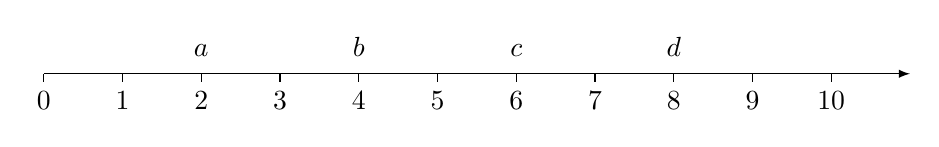
\begin{tikzpicture}
    \draw[-latex] (0,0) -- (11,0);
    \foreach \x in {0,...,10}
        \draw (\x,0) -- (\x,-3pt);
    \foreach \x in {0,...,10}
        \node [below] at (\x,-0.1) {$\x$};
    \foreach \x\y in {2/a,4/b,6/c,8/d}
        \node [above] at (\x,0.1) {$\y$};
\end{tikzpicture}
\]

\end{document}